\documentclass[11pt]{report}
\usepackage[margin=1in,footskip=0.25in]{geometry}
\usepackage[utf8]{inputenc}
\usepackage[english]{babel}
\setlength{\parindent}{4em}
\setlength{\parskip}{1em}
\usepackage{sectsty}
\usepackage{parcolumns}
\usepackage[normalem]{ulem}
%%\usepackage{showframe} % For illustration
\usepackage{tikz}
\usepackage{graphicx}
\usepackage{geometry}

% Add reference functionality
\makeatletter
\sectionfont{\ulemheading{\uuline}}
\let\oldsection\section
\newcommand{\s@section}[2][\relax]{\oldsection*{\llap{\rlap{\hspace{\textwidth}\llap{#1}}}#2}}
\makeatother


\usepackage{titlesec}
\usepackage{xcolor}
\newcommand{\mytitle}[1]{\colorbox{gray!40}{\makebox[\dimexpr\columnwidth-2\fboxsep\relax]{\filcenter #1\strut}}}
\titleformat{\paragraph}
{\normalfont\normalsize\bfseries}{\theparagraph}{1em}{\mytitle}
\titlespacing*{\paragraph} {0pt}{3.25ex plus 1ex minus .2ex}{1em}
\subsectionfont{\normalfont\large\itshape\underline}

\title{Application Project - Phase 1}
\author{J Wofford}
\date{September 2018}

\begin{document}
\raggedright

%%\maketitle

\begin{titlepage}
   \vspace*{\stretch{1.0}}
   \begin{center}
      \Large\textbf{Project: UB Room Reservation System}
      
     \vspace*{3\bigskipamount}
      \large\bfseries\textit\bigskip {Juana Wofford 1014901}
      
      \large\textit{CPSC551-Project Fall 18}
      
       \Large\textbf{PHASE 1}
       
   \end{center}
   \vspace*{\stretch{2.0}}
\end{titlepage}

\section*{Abstract}
In this paper I present developing an application in Python, MySQL and Django running on Google App Engine. Django is an open-source framework that is designed on top of Python and supports data-driven architecture.  The intent is to take advantage of Django’s rapid development and security features to quickly implement the UB Reservation System. Google App Engine provides the power and flexibility of being able to write the application code, test it locally and upload it to Google Cloud. App Engine has an automatic scaling feature that will let the application scale to meet future requirements irrespective of the number of users or the amount of data that the application stores which ensures stability. 

%%end of abstract text
\section*{Problem Statement}
The UB Room Reservation System aims to enable users to easily perform functions related to reserving a room as well as provide useful insights to the administrators, into the reservation process.  Reservations are for facilities located on the University of Bridgeport’s campus. Facilities are comprised of Meeting Rooms, Study Rooms, Study Halls and Conference Rooms.  Students, campus departments, and off-campus groups sponsoring nonprofit events can use the system. The system also allows reservations to be created for Audio / Visual Equipment and Special Events Planning. 

At present, there is not an easy way to view insights from reservation data and the reservation processes, which could be used to make the system more economically manageable and provide increased user satisfaction and usability.  The approach that will be used to fulfill this goal, is to create a application implemented in MySQL, Python and Django, using Google Cloud Computing. 
%%end of problem statement text

\paragraph{Relationships and Data Structure}

\section*{Entities}
\subsubsection{Design}
The system is organized around Room Reservations. 
\begin{itemize}
\item Reservation has a unique identifier, description name, room identifier, person who requested the reservation, service rating and the date and time for request. The creation date and creation time of the reservation is tracked. \item A reservation can be associated with any room for a specific time period.
\item A room is associated with only one active reservation for a finite time period.
\item A room has a description name, room category and room status.
\item The database will store each registered user's full name, password, email, city and state.
\item A user is identified by a unique identifier and user email.
\item A User can be of type of Admin or Normal exclusively.
\item User of type Admin can manage entire system, can access all data and run reports.
\item User of type Normal does not have any privileges of user type Admin.
\item User types of Admin and Normal can register as users, book a reservation, modify a reservation, cancel a reservation and view status of reservations.
\item User of type Normal can send messages to user of type Admin.
\item User of type Normal can rate service and quality of a reservation.
\end{itemize}

Based on the system design requirements, the following entity types are in the Reservation database:
\begin{itemize}
    \item Reservation,  Reservation Service Rating
    \item Room, Room Category, Room Status
    \item Person, User, User Category
\end{itemize}
%%end of entities design

\section*{Assumption about the database (in English)}
\subsection*{Relationships}
\begin{center}
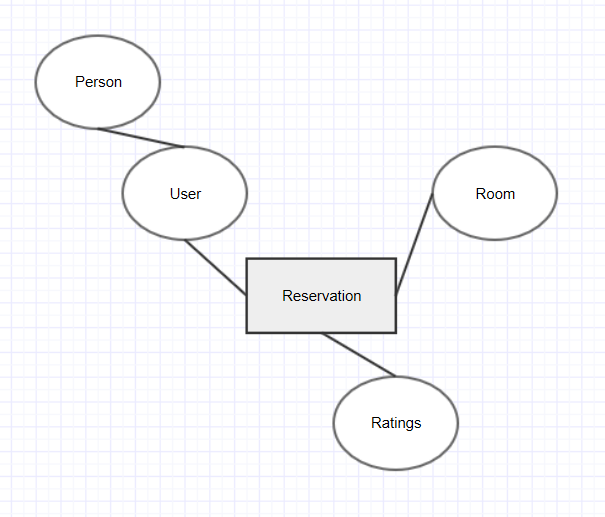
\includegraphics{reservation_conceptual.PNG}
\end{center}
\pagebreak

\subsection*{Relationship - Reservation, Room, User}
Relationship Set Example: A Reservation is created for a Room

\setlength{\parindent}{5ex}
 
 HOLDS (between RESERVATION, ROOM)
 
 
\begin{center}
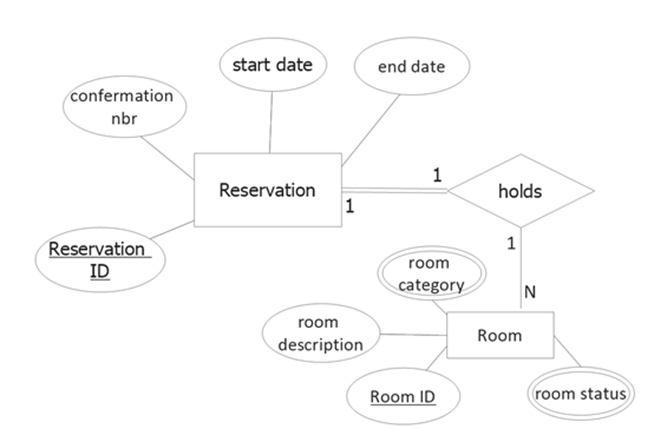
\includegraphics{resv_holds_room.PNG}
\end{center}
 
 
 
 
 

Here you talk about attributes,
 keys, the nature of relationships between entities, etc. Do not 
discuss something that is obvious (e.g.,
 that a student can take several courses). In addition,
don't make too many simplifying assumptions.


\section*{Data Queries (in English)}
\subsection*{Reservation Information}
\begin{enumerate}
\item How many Active Reservations are there in the system today?
\item How many Cancelled Reservations are there in the system today?
\item What time of day are there the most Booked Reservations?
\item What time of day are there the least Booked Reservations?
\item What User cancels the most Reservations?
\item What user modifies the most Reservations?
\end{enumerate}

\subsection*{Room Information}
\begin{enumerate}
\item What Room is the most requested?
\item What Room is the least requested?
\item What are the Rooms requested by User?
\item What type of Rooms are available for holding more than 5 people?
\end{enumerate}

\subsection*{Miscellaneous}
\begin{enumerate}
\item What are my open Reservation Requests?
\item How many times have I scheduled the 2nd Floor Conference Room?
\item What conference rooms are available at 1pm on September 6?
\item How many tables are in the 3rd Floor Study Room?
\item What Rooms, dates and times are available that have SmartBoards next month?
\end{enumerate}

\paragraph{Application Implementation Architecture}
\subsection*{Google Cloud Architecture Application}
\begin{itemize}
    \item Database - MySQL
    \item Code - Python
    \item Framework - Django
\end{itemize}

\paragraph{Conclusion - What Was Learned (Learning)}
\subsection*{Google Cloud Architecture}
    Learned differences of Google Compute Engine and Google App Engine and what each could be used for.  App Engine is used to deploy code and the platform handles its maintenance and growth.  Compute Engine is a virtual machine running in Google Cloud. It gives you more control over managing your code and applications.  Also learned that both could be used together. 
    
 \subsection*{MySQL}   
    Learning how to configure MySQL on Compute Engine. Learning how to deploy MySQL on App Engine through Python.
    
\subsection*{Database Concepts}
Learning how to apply Data Modeling Using the Entity Relationship Model for the project.


\end{document}
